
%(BEGIN_QUESTION)
% Copyright 2006, Tony R. Kuphaldt, released under the Creative Commons Attribution License (v 1.0)
% This means you may do almost anything with this work of mine, so long as you give me proper credit

A tube containing a 10 foot long column of water is angled 40$^{o}$ from horizontal.  Calculate the hydrostatic pressure at the bottom of this tube in units of inches water column ("W.C.) and also in units of atmospheres. 

$$\includegraphics[width=15.5cm]{i00234x01.eps}$$

\underbar{file i00234}
%(END_QUESTION)





%(BEGIN_ANSWER)

\noindent
{\bf Partial answer:}

\vskip 10pt

What matters here is the {\it vertical} height of the water column, not the angled length.  Essentially, this is nothing more than a problem in trigonometry: to find the length of the side opposite the 40$^{o}$ angle, given a hypotenuse of 10 feet (120 inches).

%(END_ANSWER)





%(BEGIN_NOTES)

Opposite side = (120 in)(sin 40$^{o}$) = 77.13 "W.C.

\vskip 10pt

This hydrostatic pressure is equivalent to 2.787 PSI.  Converting to PSIA we get 17.49 PSI.  Converting to atmospheres we get 1.19 Atm.


%INDEX% Physics, static fluids: hydrostatic pressure

%(END_NOTES)


